\subsection{Model \#3: Fixed primaries, varying planets and secondaries}
\label{sec:model_3}

As in the previous model, all single and primary stars in this model have 
identical properties.
The secondaries have masses, radii, and luminosities that vary between 
systems: $M\propto R \propto L^{1/\alpha}$.
The only addition is that we now let the radii of planets vary: they are 
assigned independently of any host system property, and are sampled from the 
true radius distribution, which we take as
\begin{align}
p_r(r)
&\propto
\left.
\begin{cases}
r^\delta & \text{for } r\geq 2r_\oplus \\
{\rm constant} & \text{for } r\leq2r_\oplus.
\end{cases}
\right.
\label{eq:model3_radius_distribution}
\end{align}
Following~\citet{howard_planet_2012}'s measurement, we take $\delta = -2.92$.
Our ``nominal model'' remains the same: the binary fraction is 0.44, 
$\alpha=3.5$, $\beta=\gamma=0$.
We take $Z_i$, the number of planets per single, primary, and secondary, to be 
equal.

For this model, we forgo analytic development and simply run our Monte Carlo 
program\footnote{
One might worry that our Monte Carlo program does not increase the number of 
selected stars as the square of the planet radius (Eq.~\ref{eq:snr_true}).
We can omit this dependence because in our model $N_1/N_0$ is independent of 
desired planet radius, and all other terms in the rate densities ({\it e.g.}, 
Eqs.~\ref{eq:model2_rate_density} and~\ref{eq:model2_Gamma_a}) are independent 
of the number of selected stars.
}.
The resulting occurrence rates are shown in 
Fig.~\ref{fig:errcases_model_3_log}.
For the assumed planetary and stellar distributions, the inferred rate is 
underestimated over all radii.

\begin{figure}[!tb]
    \centering
    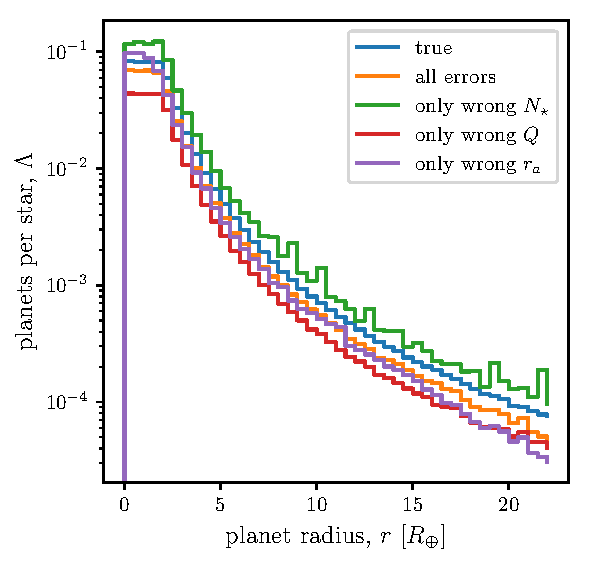
\includegraphics[width=.6\textwidth]{figures/errcases_rate_density_vs_radius_logs_model_3.pdf}
    \caption{
        Inferred planet occurrence rates as a function of planet radius in 
        Model 
        \#3.
        This model has fixed primaries and single stars, but varying 
        secondaries.
        The true planet radius distribution is a power law with exponent 
        $-2.92$ 
        above $2r_\oplus$, below which it is uniform \citep[similar 
        to][]{howard_planet_2012}.
    }
    \label{fig:errcases_model_3_log}
\end{figure}

\paragraph{Hot Jupiter occurrence rates}
Taking Fig.~\ref{fig:errcases_model_3_log} and counting the number of planets 
per star with $r>8r_\oplus$, we can compare the true and inferred hot Jupiter 
occurrence rates.
Under the above assumptions, the true rate is 9.1 hot Jupiters 
per thousand stars.
The inferred rate is 6.9 per thousand stars.
This means that the inferred rate underestimates the true rate by a 
multiplicative factor of $\sim\!1.3$.

However, this result only applies under the assumption that $Z_0 = 
Z_1 = Z_2$.
If hot Jupiters are less common around lower mass stars, it would be more 
sensible to consider $Z_2<Z_0$, while letting single stars and 
primaries host planets at the same rate.
Therefore in Fig.~\ref{fig:HJ_correction_inputrate_vs_HJratevalues} we let 
$Z_2$ vary, and show the resulting inferred and true hot Jupiter 
($r>8r_\oplus$) rates.
The result is that the inferred rate is nearly independent of 
$Z_2$~--~this is because most ($<1/10$) secondaries are not searchable, 
and so their completeness fraction is much smaller than that of primaries or 
single stars.
This means far fewer detected hot Jupiters orbit secondaries, and so they 
hardly affect the inferred rate.
While the ``true rate'' across the entire population is linearly dependent on 
$Z_2$, the rate around 
singles and primaries (Fig.~\ref{fig:HJ_correction_inputrate_vs_HJratevalues} 
green line) is independent of that around secondaries.

\begin{figure}[!tb]
    \centering
    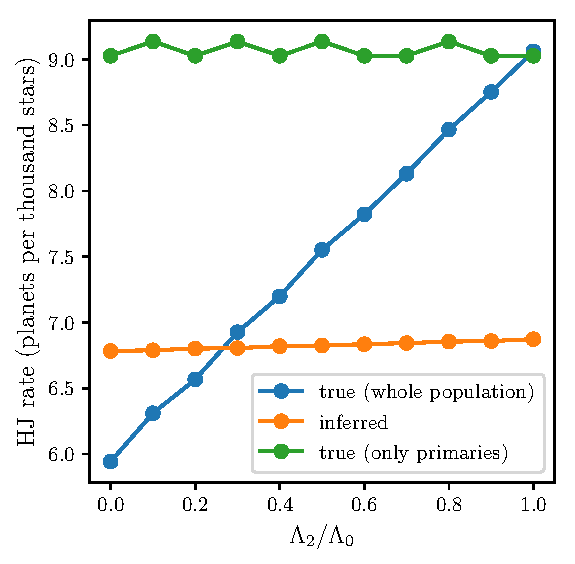
\includegraphics[width=.6\textwidth]{figures/HJ_correction_inputrate_vs_HJratevalues.pdf}
    \caption{
        $Z_i$ is the occurrence rate integrated over all possible phase 
        space for the $i^{\rm th}$ system type. $Z_2/Z_0=1$ 
        corresponds to an equal number of planets per secondary as per single 
        star;
        $Z_2/Z_0=0$ corresponds to secondaries not having any 
        planets.
        In our Model \#3, though the true HJ occurrence rate 
        is highly dependent on $Z_2$, 
        the inferred rate hardly depends on whether secondaries have HJs.
        This means that the ``correction factor'' between the inferred rate 
        and the true rate around single stars is underestimated by a 
        multiplicative 
        factor of $\approx1.3$, independent of the HJ rate around secondaries.
        The ``HJ rate'' is the summed rate from     
        Fig.~\ref{fig:errcases_model_3_log} above $8r_\oplus$.
    }
    \label{fig:HJ_correction_inputrate_vs_HJratevalues}
\end{figure}


\paragraph{The rate of Earth analogs}
This model provides an estimate of the apparent and true 
rates as a function of radius (Fig.~\ref{fig:errcases_model_3_log}).
At Earth's radius, the result is that the inferred rate is $0.84\times$ the 
true rate around single stars, assuming that the $Z_i$'s are equal.
Similar to the above case of the hot Jupiters, if we vary the true $Z_2$ 
while keeping $Z_0 = Z_1$, the ratio of the inferred to true rate 
around single stars changes by only a few percent (shown in 
Fig.~\ref{fig:earth_inputrate_vs_etaearthratevalues}).
The ratio of the inferred to the true rate, $(\Lambda_{\rm 
    inferred}/\Lambda)_{r=r_\oplus}$ varies substantially, but by at most 
    $50\%$ 
in the (unrealistic) limiting case that secondaries do not host planets.


\begin{figure}[!tb]
    \centering
    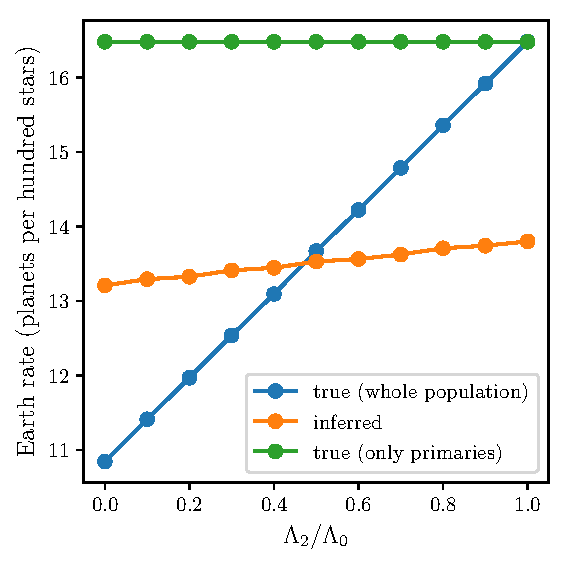
\includegraphics[width=.6\textwidth]{figures/earth_inputrate_vs_etaearthratevalues.pdf}
    \caption{
        Same as Fig.~\ref{fig:HJ_correction_inputrate_vs_HJratevalues}, but 
        for Earth-sized planets.
        The absolute values given on the $y$-axis found by summing the rate 
        from Fig.~\ref{fig:errcases_model_3_log} for planetary radii from 
        $0.5$ to $1.5r_\oplus$ (this is a toy model, and they do not reflect 
        an actual determination of $\eta_\oplus$).
        The relative values show that the inferred rate for Earths is roughly 
        independent of the occurrence rate (integrated over all radii) around 
        secondaries.
        However, it is systematically lower than the true rate around single 
        and primary stars, by $\approx 20\%$.
    }
    \label{fig:earth_inputrate_vs_etaearthratevalues}
\end{figure}